\section{Transformers in Reinforcement Learning}
Transformers, originally developed for sequence modeling in natural language processing, have attracted growing interest in 
reinforcement learning (RL) due to their ability to capture long-range dependencies and handle complex sequential data. In the 
following sections, we will first explore the core mechanisms of the transformer architecture, and then discuss how the standard 
transformer is adapted for use in RL. However, we will not delve deeply into specific RL papers that apply transformers.
At a high level, the process of how an input is processed by a transformer can be broken down into a series of steps: \newline
\vspace{-0.8cm}
\begin{wrapfigure}[16]{r}{5.5cm}
    \caption{Transformer architecture from \cite{vaswani2023attentionneed}}
    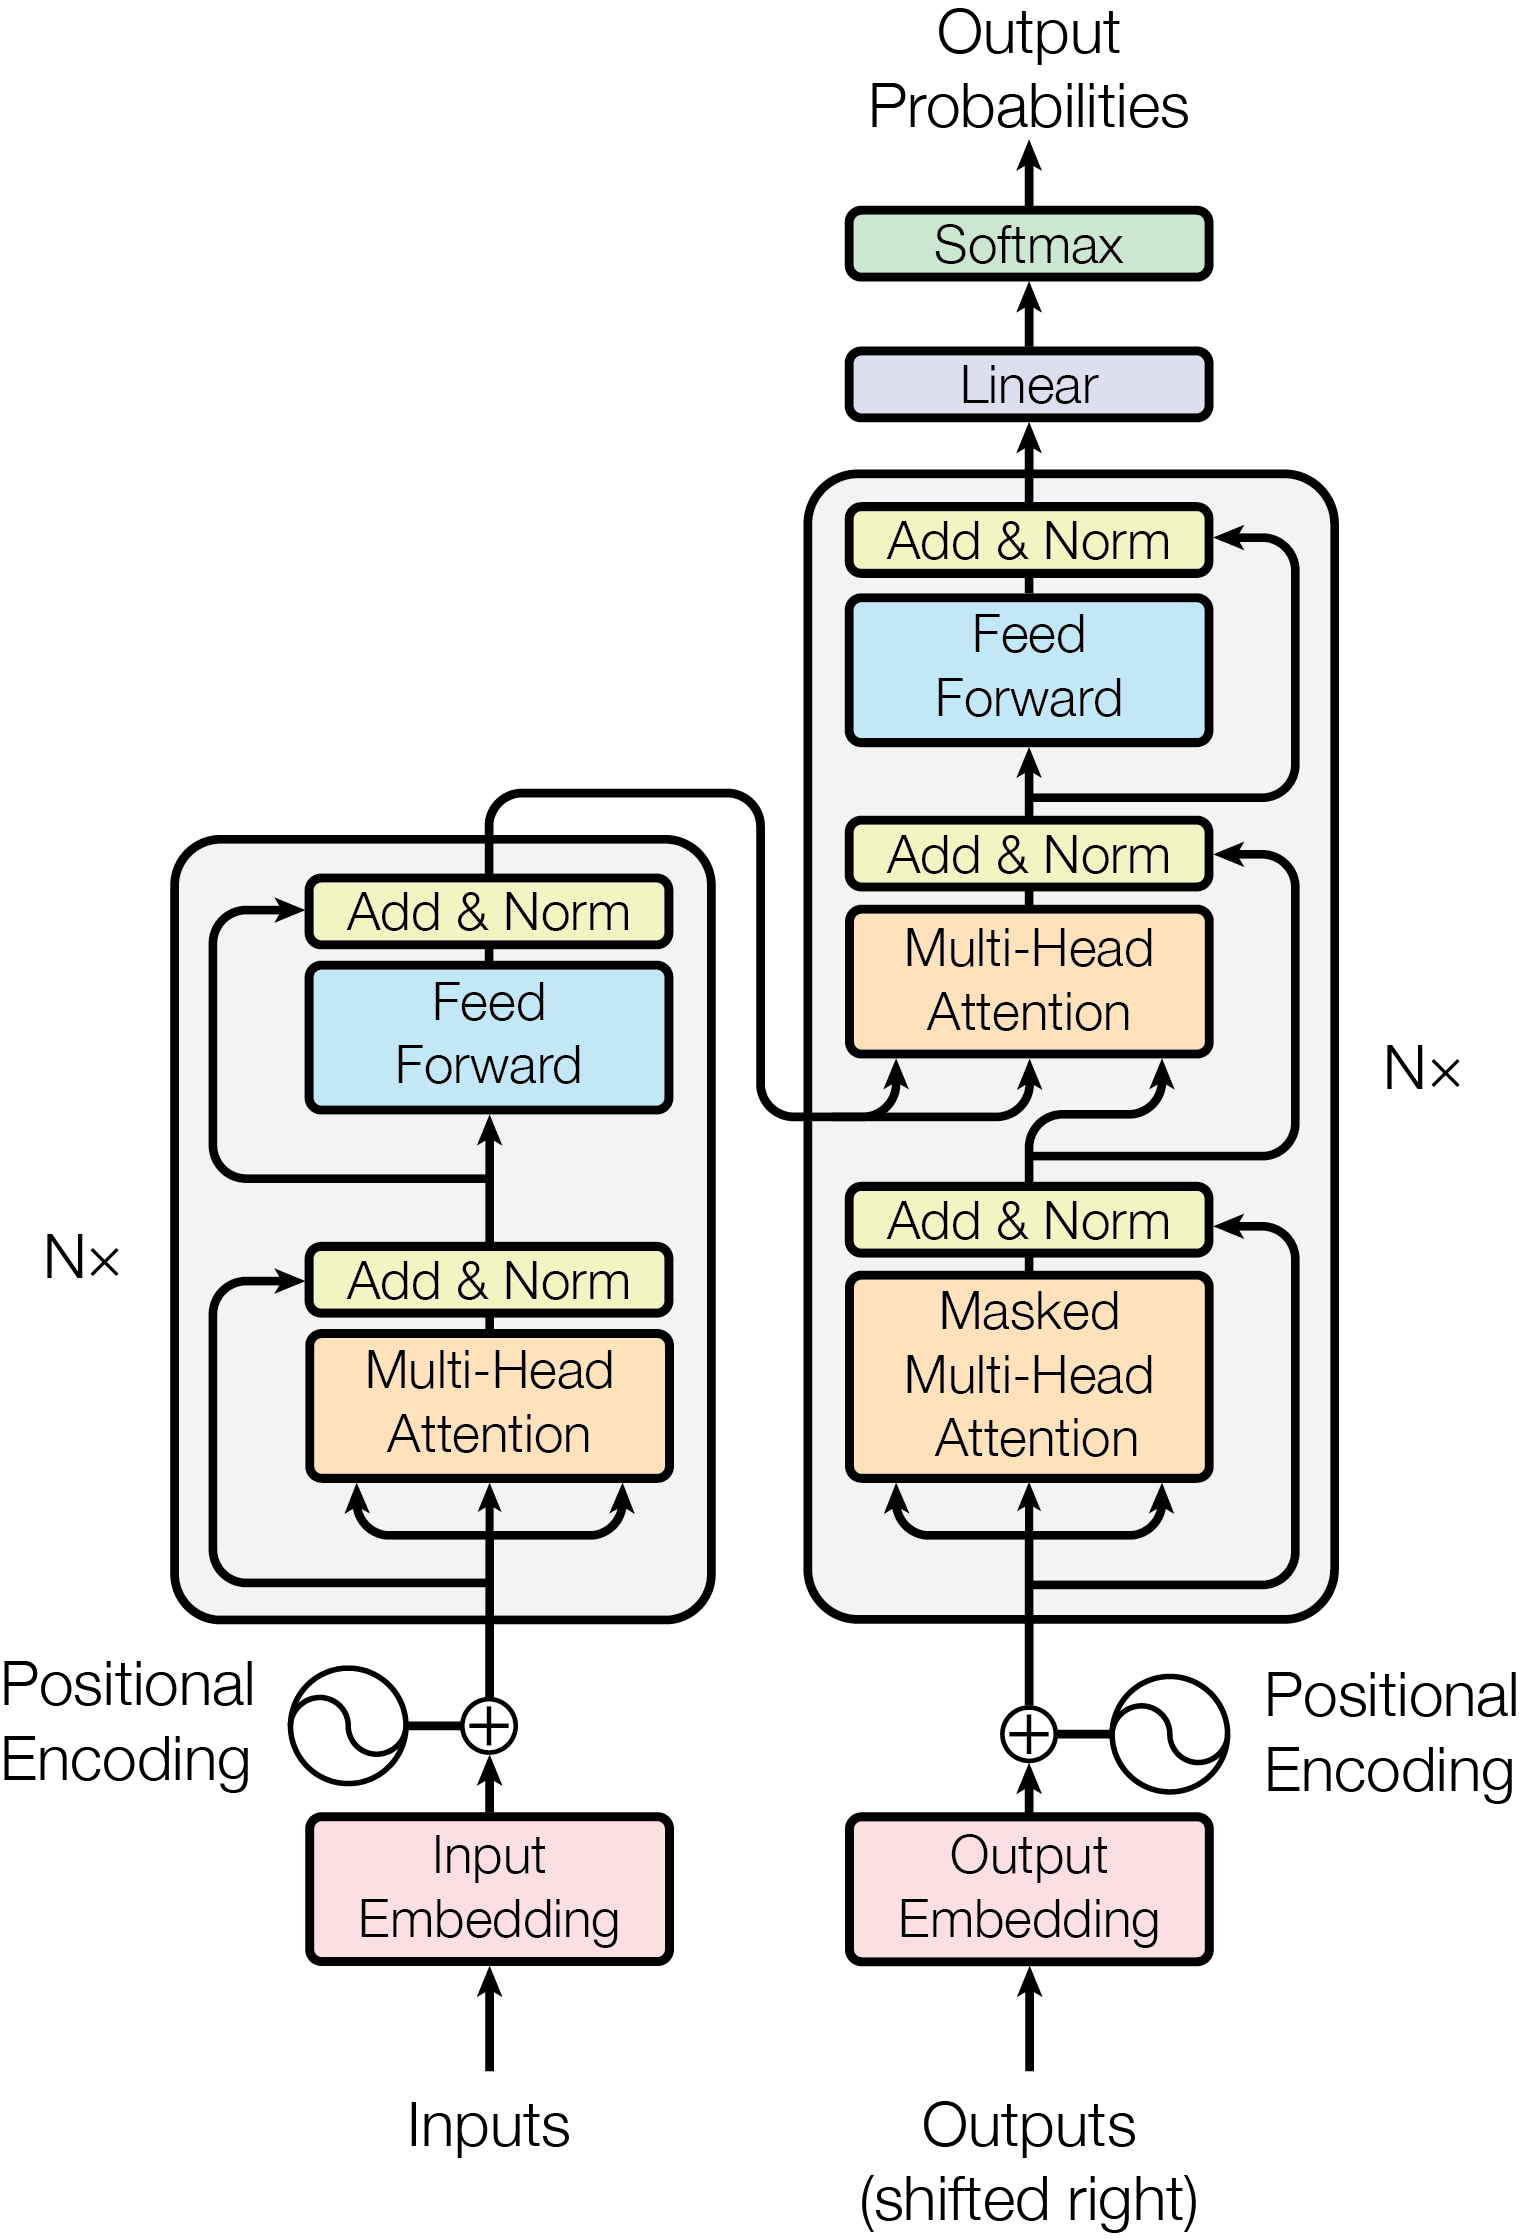
\includegraphics[height=10cm]{images/ModalNet-21.png}
    \label{transformer}
\end{wrapfigure}
\begin{enumerate}
\item \textbf{Input Embedding:} Converts input tokens or data into dense vector representations. In NLP, this applies to 
words/tokens; in RL or vision tasks, states or images are embedded.

\item \textbf{Positional Encoding:} Adds position information to embeddings, allowing the transformer to capture sequence 
order, which it doesn't handle inherently.

\item \textbf{Self-Attention Mechanism:} Enables each token to attend to all others using learned query, key, and value 
vectors. Attention scores—based on query-key similarity—determine how much focus each token gives to others, producing a 
weighted sum of values.

\item \textbf{Feedforward Network:} Applies a fully connected neural network to each position independently for further 
transformation.

\item \textbf{Residuals \& Layer Norm:} Residual connections and layer normalization follow attention and feedforward layers 
to stabilize training and preserve information.

\item \textbf{Stacked Layers:} Multiple layers refine the representations, allowing deeper abstraction and more complex 
understanding.

\item \textbf{Output:} Final outputs vary by task—e.g., softmax classification in NLP or decision-making in RL.
\end{enumerate}
%\begin{enumerate}
%\item  Input Embedding: The input is first converted into embeddings. For NLP tasks, this might involve 
%converting words or tokens into dense vector representations. In other applications, such as RL or image 
%processing, this could involve encoding states or images into suitable embeddings.

%\item Positional Encoding: Since transformers don't inherently capture the order of the input sequence (like 
%RNNs or LSTMs), positional encodings are added to the embeddings to inject information about the position of 
%each element in the sequence. These encodings are usually vectors that represent the position of tokens in 
%the sequence.

%\item Self-Attention Mechanism: The key feature of the transformer is the self-attention mechanism. For each 
%element in the sequence (e.g., word or state), the model computes attention scores with respect to all other 
%elements in the sequence. This allows each token to "attend" to every other token, enabling the model to 
%capture relationships and dependencies across the entire sequence.

%\item Attention Scores and Weighted Sum: The attention mechanism calculates a weighted sum of all input 
%embeddings based on how much focus each token should have on others. This is done using three learned vectors 
%per token: queries, keys, and values. The attention score between two tokens is calculated as the similarity 
%between their query and key vectors.

%\item Feedforward Neural Networks: After the self-attention step, each token's representation is passed 
%through a feedforward neural network. This helps further process the information and allow for more complex 
%transformations of the input sequence.

%\item Residual Connections and Layer Normalization: To prevent the model from losing information through deep 
%layers, transformers use residual connections around both the attention and feedforward layers, followed by 
%layer normalization. This helps stabilize training.

%\item Multiple Layers: The transformer consists of multiple layers of attention and feedforward networks. 
%Each layer refines the input, allowing the model to capture increasingly complex relationships between tokens 
%or elements in the sequence.

%\item Output: The final output of the transformer can be processed in various ways, depending on the task. 
%For instance, in NLP tasks, the output might be passed through a softmax layer for classification, or in RL, 
%it might inform the next action or state prediction.

%\end{enumerate}
\noindent
In the following, we will take a closer look at the individual steps, primarily focusing on 
language processing. However, it's important to note that transformers are not limited to 
language—they can also process other types of inputs, such as images. We focus on language 
processing here simply because it's a clear and intuitive way to understand the core steps 
of how transformers work.

\subsection{Embedding}
The first stage in training a transformer model involves converting raw input into vector representations—a process known as 
input embedding. A basic approach to representing words is one-hot encoding, where each word is assigned a binary vector the 
size of the vocabulary, with a single 1 indicating the presence of that word and 0s elsewhere. Although simple, this method 
has significant drawbacks: the vectors are high-dimensional, sparse, and fail to capture any semantic relationships between 
words.\newline 
To address these limitations, learned word embeddings are used. These are dense, low-dimensional vectors trained to capture 
semantic meaning, typically using unsupervised learning techniques. Words with similar meanings are mapped to similar vector 
representations. For example, the vectors for “queen” and “woman” will lie close in the embedding space due to shared 
contextual usage. Embeddings can also reflect relationships, such as vector arithmetic:
$$\text{vector(queen)}\approx \text{vector(king)}+\text{vector(woman)}-\text{vector(man)} $$
\begin{figure}[H]
    \centering
    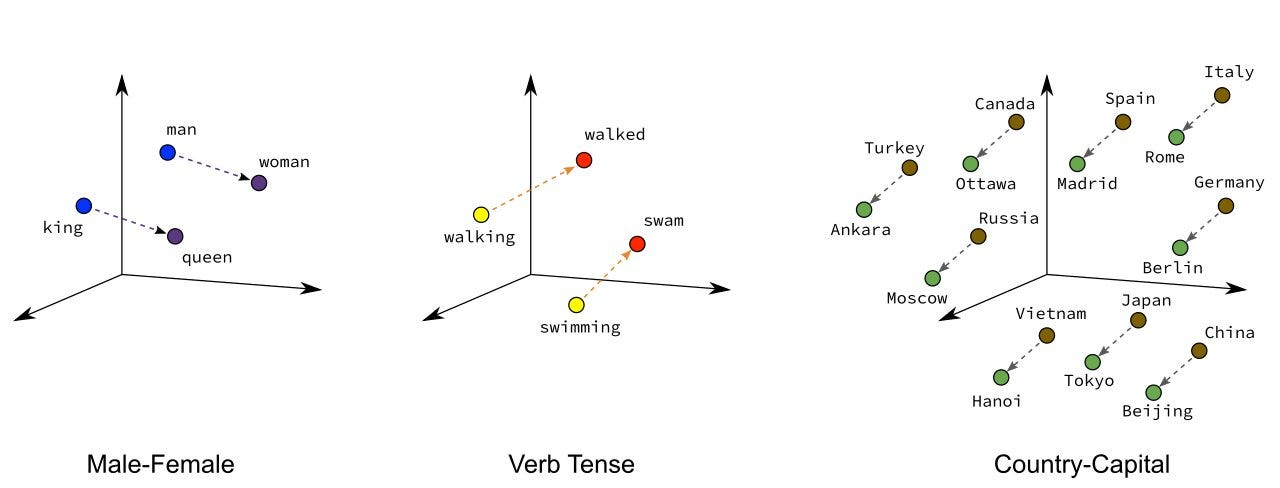
\includegraphics[width=0.8\linewidth]{images/embeddings.jpg}
    \caption{Illustration of potential embeddings, Image from \cite{WordVectors}}
    \label{embeddings}
\end{figure}
Importantly, these embeddings extend beyond representing words in isolation—they evolve through the layers of a transformer to
reflect contextual meaning. For instance, the embedding of “mathematician” could shift to refer specifically to Leibniz, 
depending on the sentence context. While the initial embedding layer does not yet account for surrounding context, it provides 
a foundational semantic representation that is refined throughout the transformer architecture.
(While there are several types of embedding techniques, such as Word2Vec and GloVe, we will not explore them in detail here.)

\subsection{Positional Encoding}
The position of words in a sentence plays a crucial role in understanding their meaning. Early models, such as Recurrent 
Neural Networks (RNNs), inherently capture word order through their sequential processing. However, the Transformer 
architecture does not process tokens sequentially, and therefore lacks an inherent sense of word order. To address this, 
positional encoding is introduced to inject information about the position of each token in the sequence. An effective 
positional encoding scheme should satisfy the following criteria:
\begin{itemize}
    \item \textbf{Unambiguous:} Each position in the sequence should have a unique encoding.
    \item \textbf{Deterministic:} It is beneficial if the encoding follows a predictable mathematical pattern, allowing the 
    model to learn or infer position-based relationships.
    \item \textbf{Distance-aware:} The encoding should enable the model to estimate the relative distance between two 
    positions.
    \item \textbf{Generalizable:} The encoding should allow the model to handle longer sequences than those seen during 
    training. Ideally, values should be bounded to avoid numerical instability.
\end{itemize}
The authors of the \textit{Attention is All You Need} paper \cite{vaswani2023attentionneed} define positional encoding using 
sinusoidal functions as follows:
\begin{gather*}
    f(t)_i = \begin{cases}
        \sin{(\omega_k \cdot t)}, \quad \text{if } i= 2k\\
        \cos{(\omega_k \cdot t)},  \quad \text{if } i= 2k+1
        \end{cases} = \begin{bmatrix}
            \sin{(\omega_{1}\cdot t)} \\
            \cos{(\omega_{1}\cdot t)}\\
            \sin{(\omega_{2}\cdot t)} \\
            \vdots \\
            \sin{(\omega_{d/2}\cdot t)} \\
            \cos{(\omega_{d/2}\cdot t)}\\
         \end{bmatrix}_{d\times 1} \\ 
         \text{with } \omega_k = \frac{1}{10000^{2k/d}}
\end{gather*}
Here, $t$ denotes the position of a token in the sequence (e.g., the 1st, 2nd, or 3rd word), and $d$ is the dimensionality of 
the embedding space. Each dimension of the positional encoding corresponds to a sinusoid with a different frequency.\newline
This encoding is unique as long as the chosen frequencies span a range that exceeds the maximum sequence length $L$ 
(where $t \in \{1, \dots, L\}$). Put simply, at least one dimension must have a sinusoid whose period exceeds $L$, ensuring that 
the function values do not repeat and each position maps to a distinct representation.  Since sine and cosine are 
deterministic functions, the positional encoding is also deterministic. Furthermore, the sinusoidal encoding generalizes well to 
sequences longer than those seen during training, thanks to the periodic nature of sine and cosine functions. Finally, this 
encoding is distance-aware. Because each dimension of the encoding uses a different frequency, the model can infer relative 
positions from the differences between encodings.

\subsubsection{Binary Representation and Positional Encoding}
The intuition behind sinusoidal positional encoding becomes clearer when we consider the binary representation of numbers. At 
first glance, one might wonder how a combination of sine and cosine waves can meaningfully represent position or order. The 
answer lies in how binary counting works.
\begin{figure}[H]
    \centering
    \begin{minipage}[t]{0.25\textwidth}
     \vspace{2cm}
        \centering
        \begin{tabular}{c|c}
        \textbf{0:} 0000 & \textbf{8:} 1000 \\
        \textbf{1:} 0001 & \textbf{9:} 1001 \\
        \textbf{2:} 0010 & \textbf{10:} 1010 \\
        \textbf{3:} 0011 & \textbf{11:} 1011 \\
        \textbf{4:} 0100 & \textbf{12:} 1100 \\
        \textbf{5:} 0101 & \textbf{13:} 1101 \\
        \textbf{6:} 0110 & \textbf{14:} 1110 \\
        \textbf{7:} 0111 & \textbf{15:} 1111 \\
        \end{tabular}
    \end{minipage}%
    \hfill
    \begin{minipage}[t]{0.75\textwidth}
     \vspace{0pt}
        \centering
        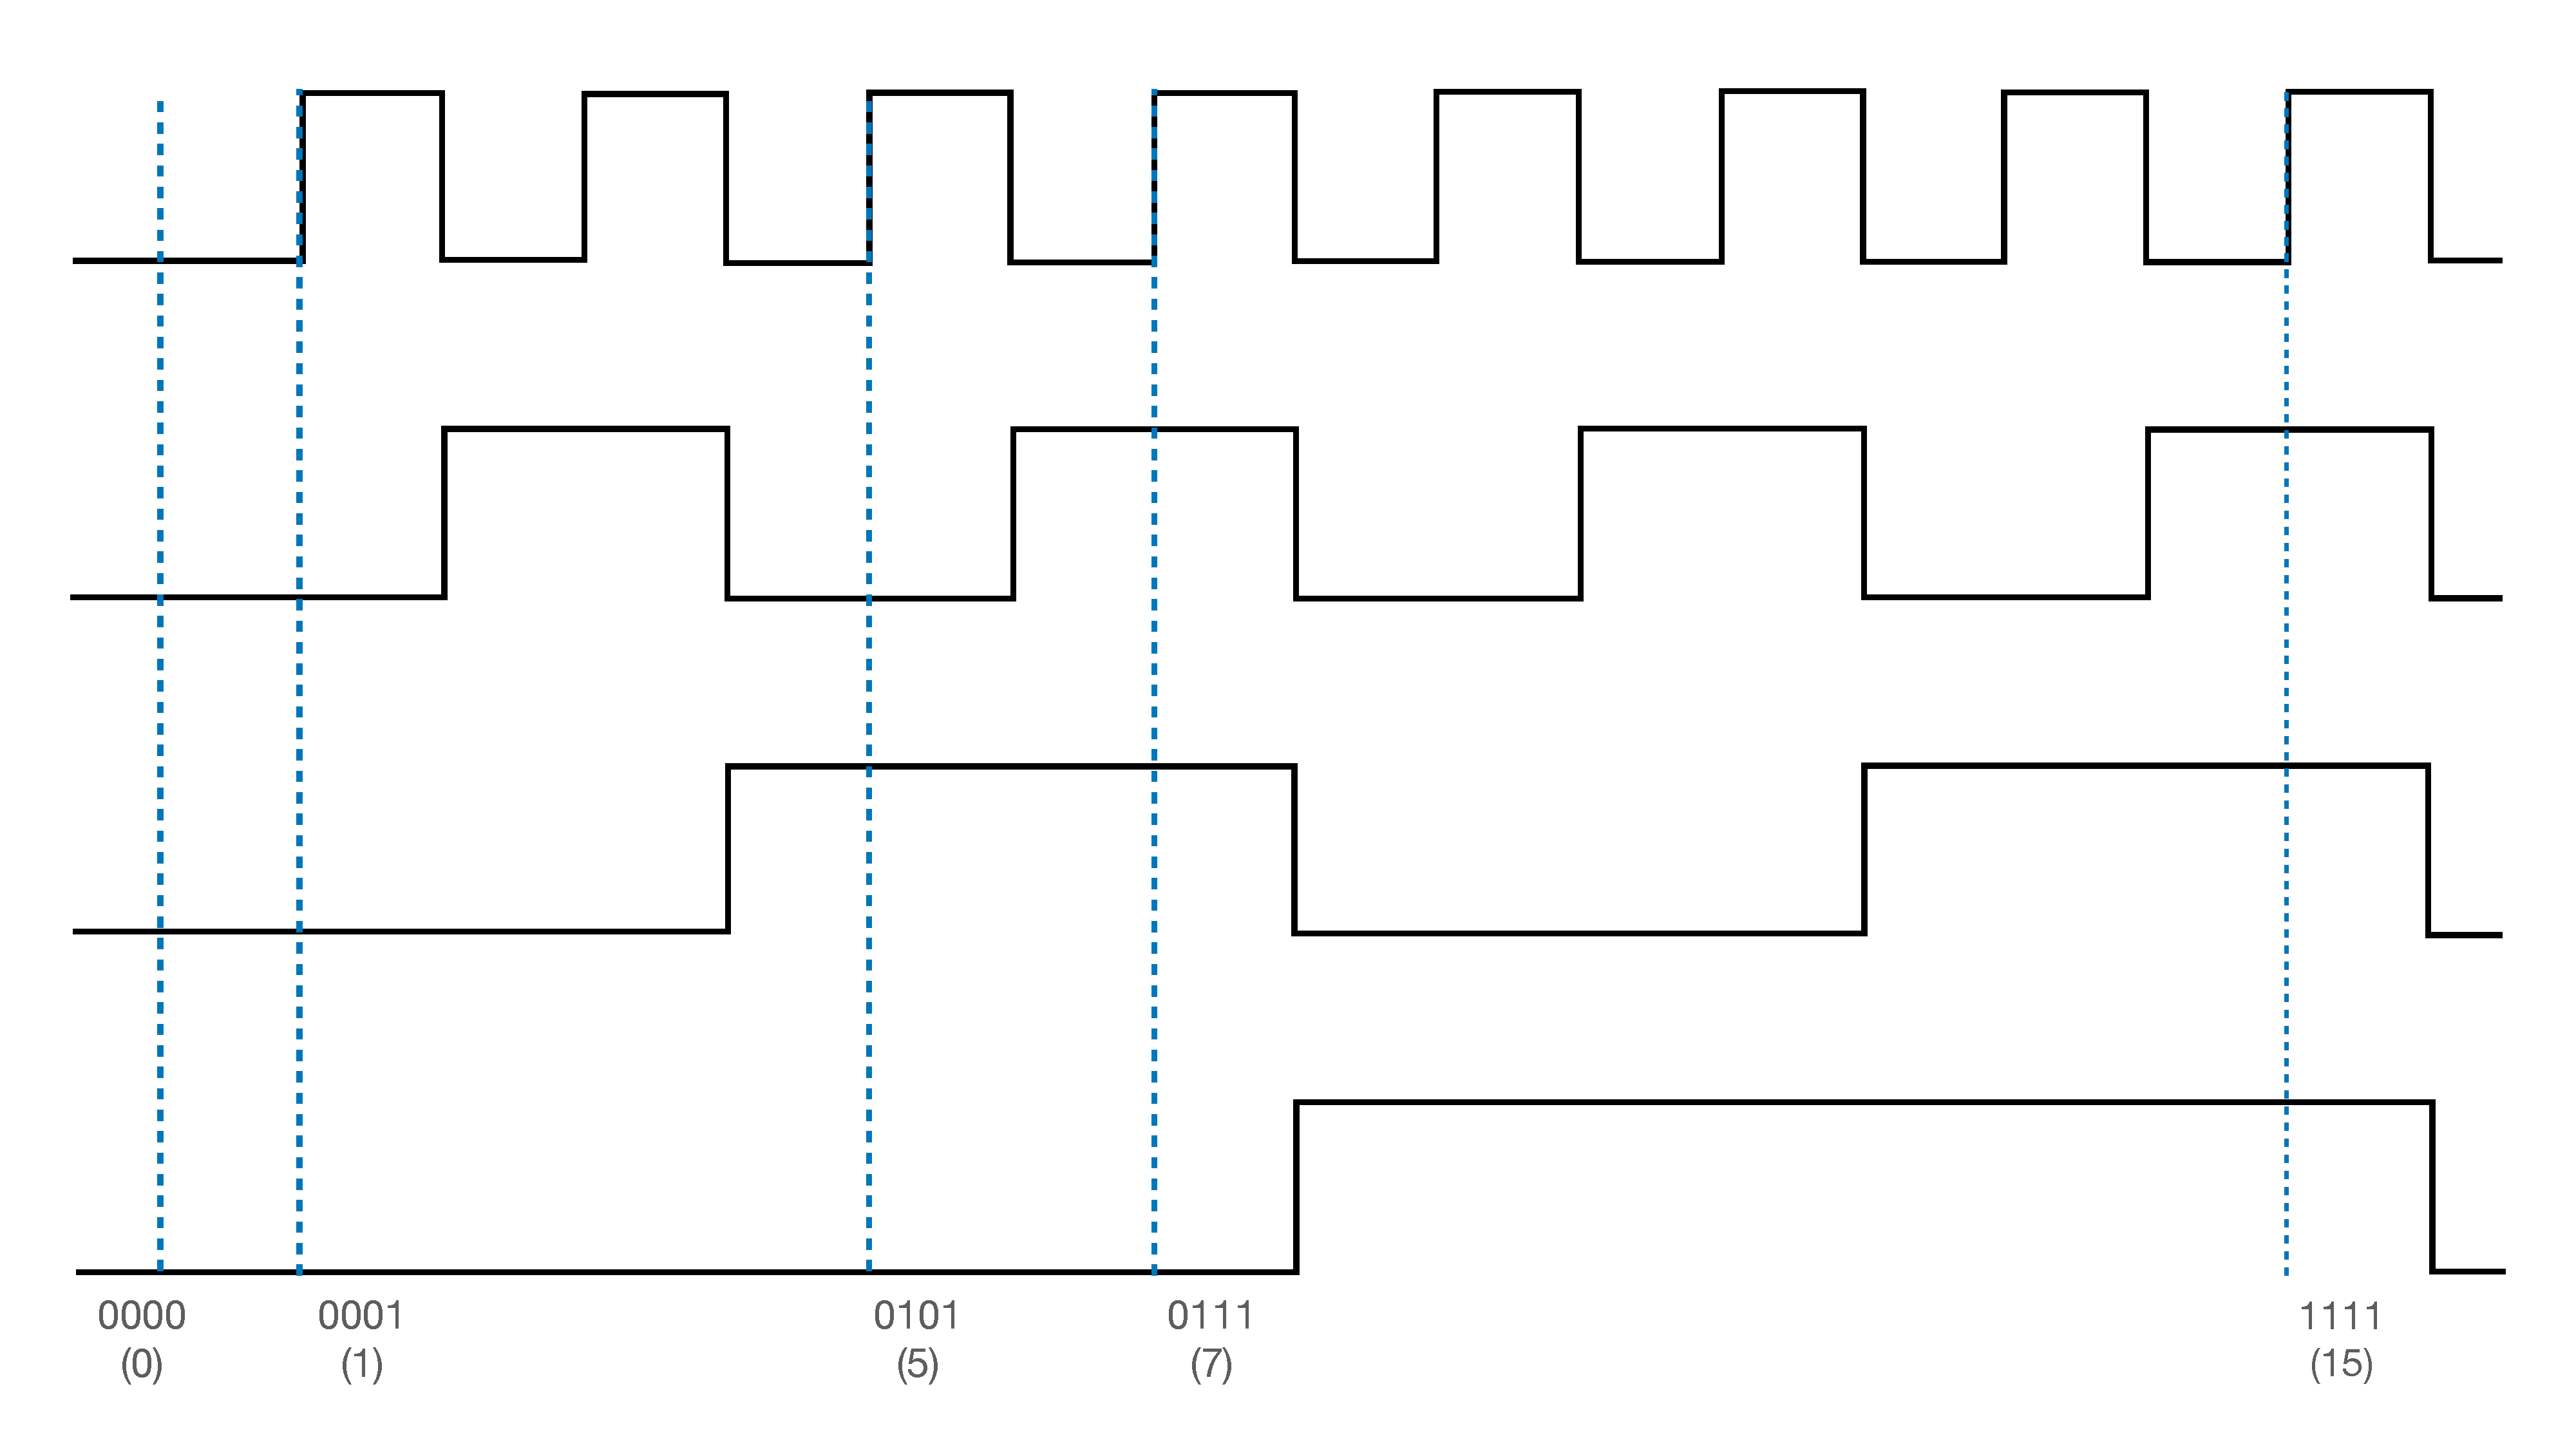
\includegraphics[width=\linewidth]{images/4_bit_counter.pdf}
        %\caption{4-bit binary counter waveform visualization.}
        \label{fig:4bit-counter}
    \end{minipage}
    \caption{Illustration of the 4-bit binary number system. On the left is the binary representation in tabular form, and on 
    the right is a visualization using periodic step functions (square waves).}
\end{figure}
\vspace{-0.3cm}
So, we can use periodic wave functions (one for each dimension) to encode numbers. This idea closely resembles the sine and 
cosine functions used in positional encoding. Using discrete binary values directly would be inefficient in the continuous 
space of neural networks. Instead, we use their smooth, differentiable counterparts: sinusoidal functions. These functions act 
as continuous analogues of alternating bits. By varying their frequencies we mimic the behaviour of binary bits flipping at 
different rates. This allows the model to infer both absolute position and relative distance, all within a compact and expressive 
representation.
\begin{figure}[H]
\hspace{1.5cm}
    %\centering
    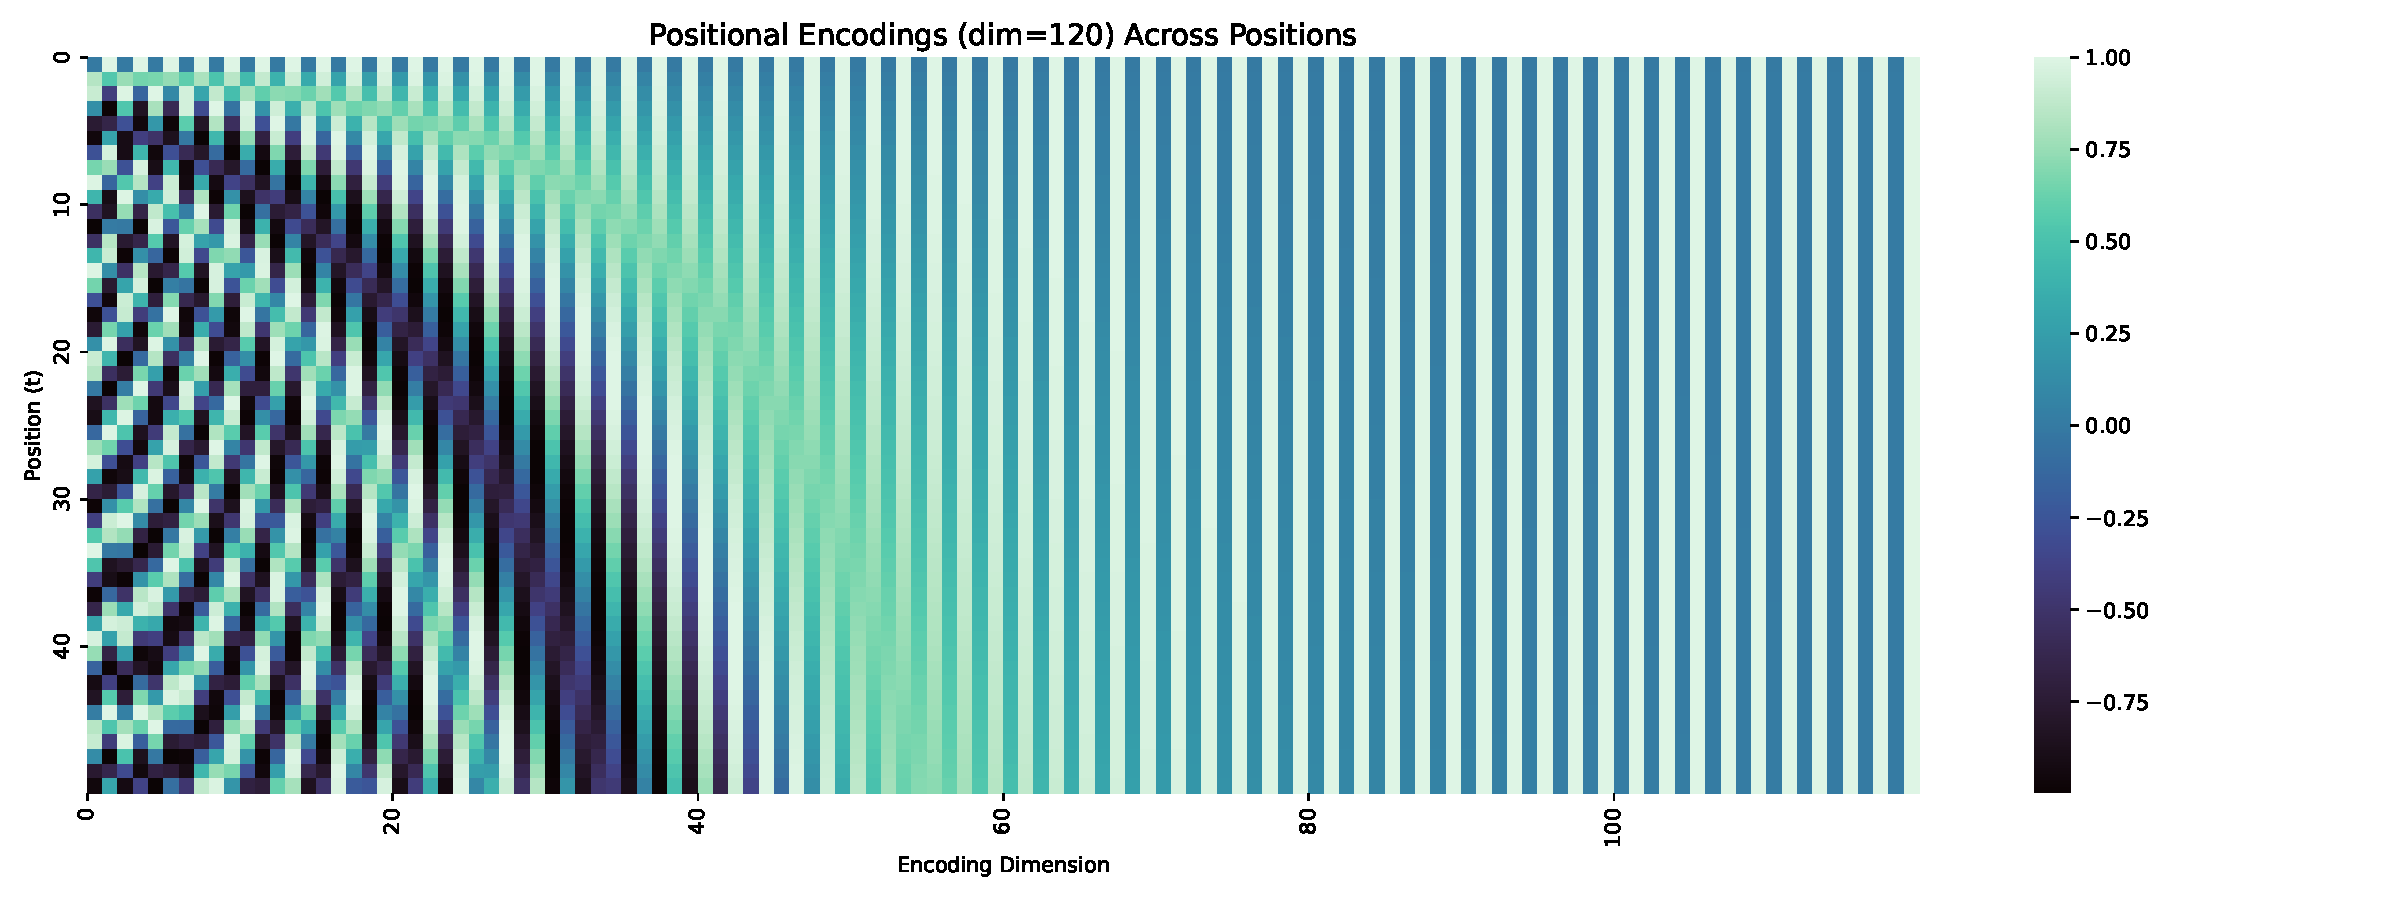
\includegraphics[width=0.92\linewidth]{images/pos_enc_visual.pdf}
   \caption{Visualization of positional encodings for positions 0 to 49 with an encoding dimension of 120. Each row represents 
   the positional encoding for one position, and each column corresponds to a specific dimension with its associated value.}
    \label{fig:pos_enc_vis}
\end{figure}
\subsection{Attention Mechanism}
In a transformer model, the key objective is for embeddings (vectors) to not only represent individual words 
but also capture context, allowing for a more nuanced understanding of language. This is achieved through 
the self-attention mechanism. To understand this, let's first break down a simple example and build on it.
Let's consider a sentence like ''Kings made laws to keep power over the small towns`` and focus on how the 
attention mechanism works. Each word is initially represented as an embedding vector $\vec{E}_i$.

\subsubsection{Query, Key, and Value Vectors}
From each embedding $\vec{E}_i$, three vectors are computed using learned weight matrices: 
\begin{itemize} 
\item $\vec{Q}_i = W_Q \vec{E}_i$ (Query) 
\item $\vec{K}_i = W_K \vec{E}_i$ (Key) 
\item $\vec{V}_i = W_V \vec{E}_i$ (Value) 
\end{itemize}
These vectors will determine how a token attends to others in the sequence.

\subsubsection{Attention Scores}
The next step is to measure the relevance of the different tokens in relation to each other. This is done by 
computing the dot product between the query vector of one word and the key vectors of all other words. The 
dot product gives a measure of similarity: high positive value indicates that the two words are more relevant to 
each other in the context (vectors pointing in nearly the same direction) while negative values indicate that the words
are not so relevant to each other (vectors nearly pointing in opposite directions).

\subsubsection{Softmax}
After computing the dot product, we apply a softmax operation to the values. This converts the raw scores 
into probabilities, allowing the model to focus more on the most relevant words and ignore less relevant 
ones.\newline
Additionally, in some settings (e.g., in reinforcement learning), we may mask certain values in the 
attention matrix, ensuring that later words do not influence earlier ones. This is done by setting specific
values to negative infinity before applying softmax, which effectively eliminates their contribution.

\subsubsection{Updating the Embedding}
Now that we know which words are important for each other, the next step is to update the embeddings. The 
update is based on the value matrix, which is another learned weight matrix. The value matrix is multiplied 
by each word’s embedding, and the resulting vectors are summed to produce the final output.\newline
The value matrix answers the question: If this word is relevant to adjusting the meaning of another word, what specific adjustments should be made? This results in a new set of embeddings that reflect the context. The whole attention procedure 
can be described via the function $$\text{Attention}(Q,K,V) = \text{softmax}\left(\frac{QK^T}{\sqrt{d_k}}\right)V$$
To understand why the attention scores are scaled by $\sqrt{d_k}$, consider the dot product between a 
query vector $\vec{q}_i$ and a key vector $\vec{k}_j$:
$$\sigma_{ij} = \vec{q}_i \cdot \vec{k}_j = \sum_{n=1}^{d_k} q_{in} k_{jn}$$
If we assume that the components of $\vec{q}_i$ and $\vec{k}_j$ are independent, have zero mean, and unit variance (we can 
make the assumption due to the use of LayerNorm), then each term in the sum $q_{in} k_{jn}$ will have mean zero and variance 
1. Therefore, the variance of the sum (i.e., the dot product) becomes:
$$\text{Var}(\sigma_{ij}) = \sum_{n=1}^{d_k} \text{Var}(q_{in} k_{jn}) = d_k \longrightarrow 
\text{std}(\alpha_{ij}) = \sqrt{d_k}$$
This means the standard deviation of the attention score grows with the square root of the key dimension. The normalization 
ensures that the variance of the attention scores remains approximately constant, regardless of dimensionality, leading to 
more stable gradients and more effective learning.
\begin{figure}[H]
  \centering
  \begin{minipage}[b]{0.45\linewidth}
    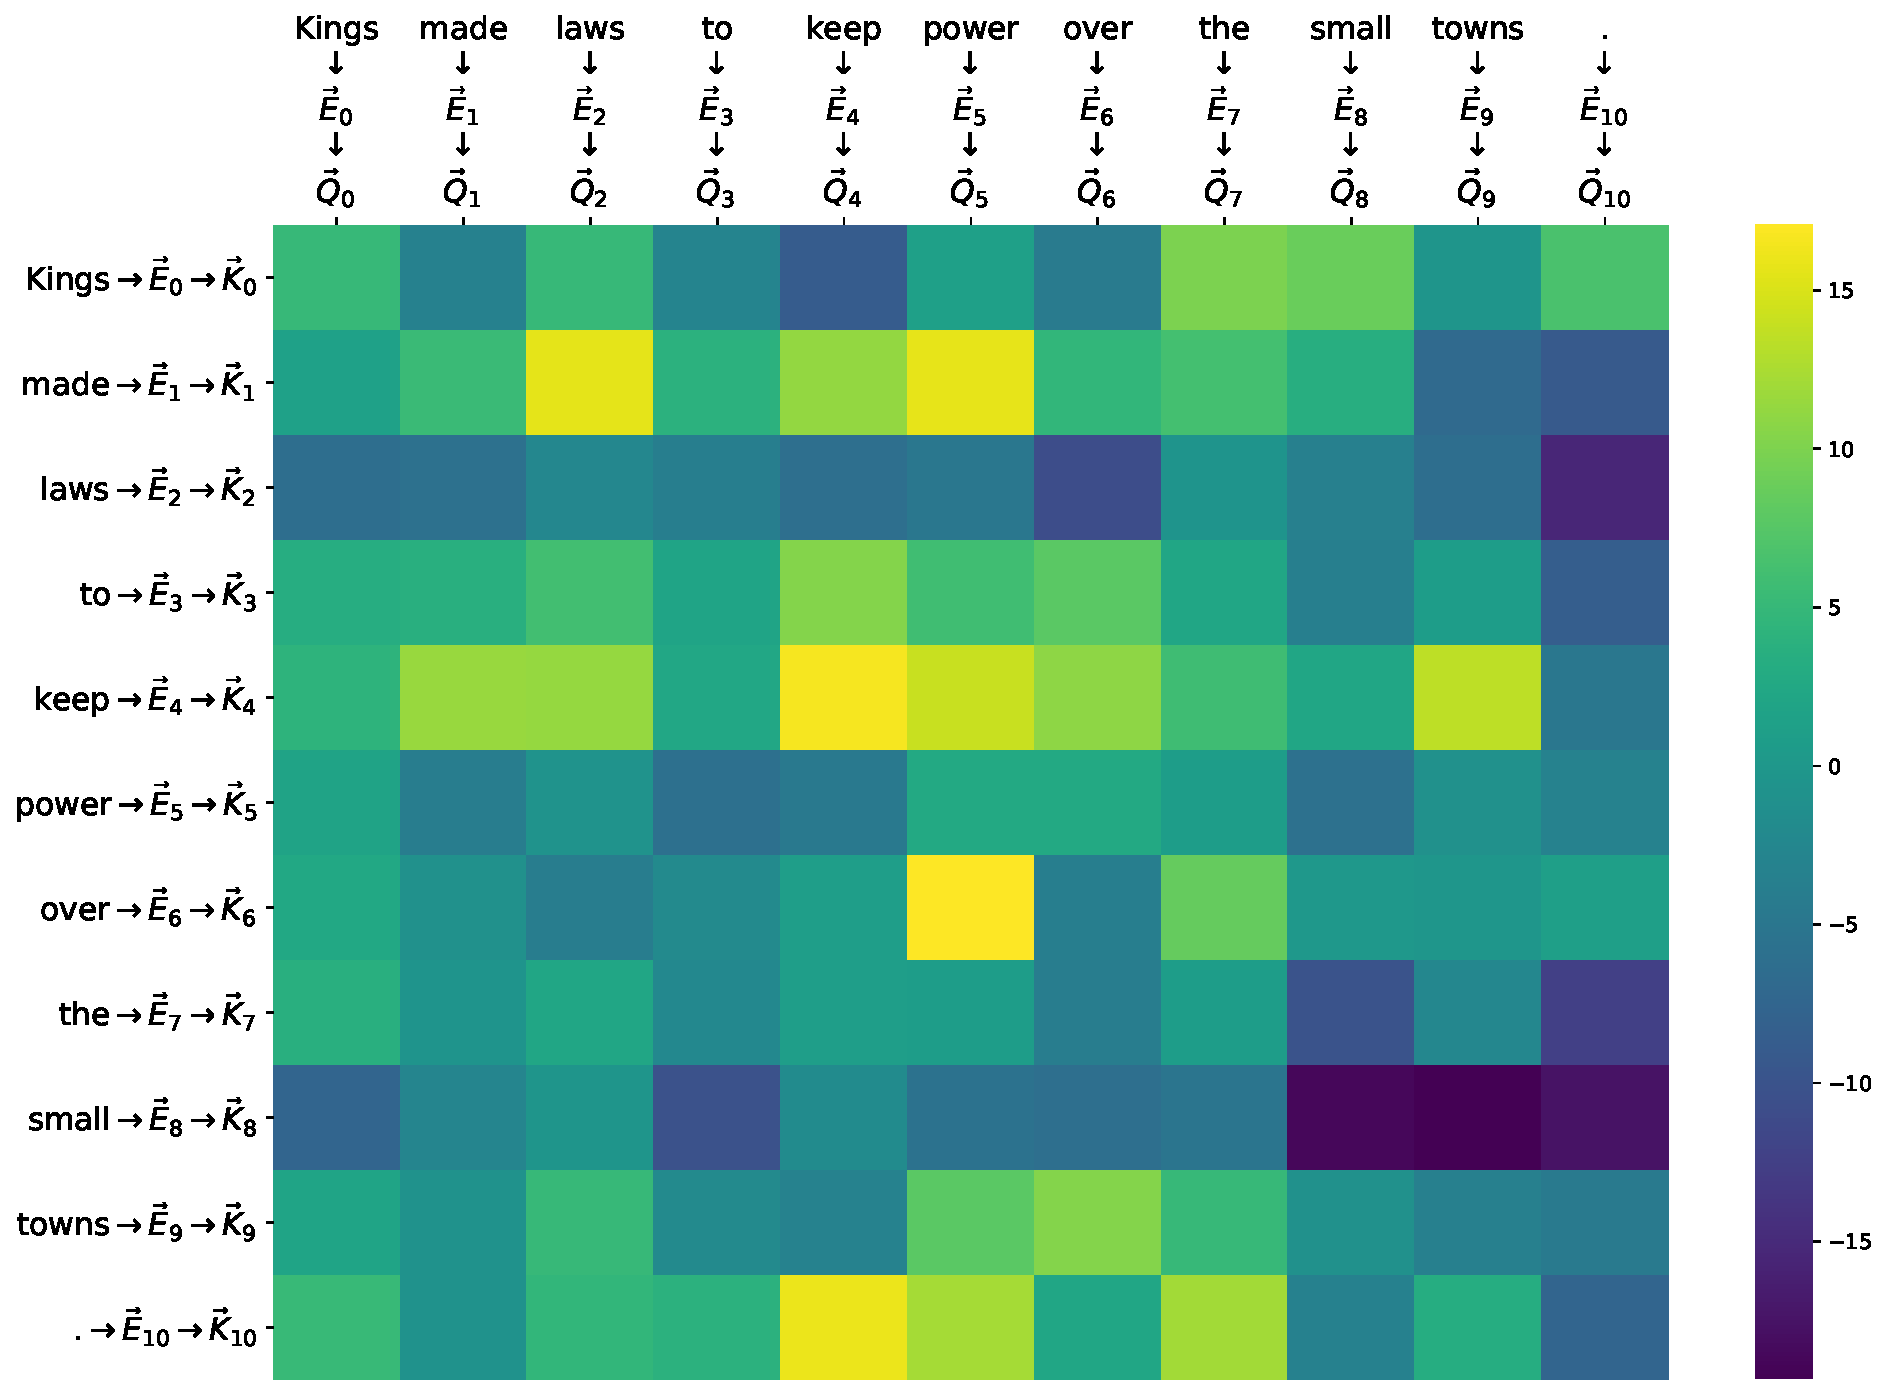
\includegraphics[width=\linewidth]{images/normal_attn.pdf}
  \end{minipage}
  \hfill
  \begin{minipage}[b]{0.45\linewidth}
    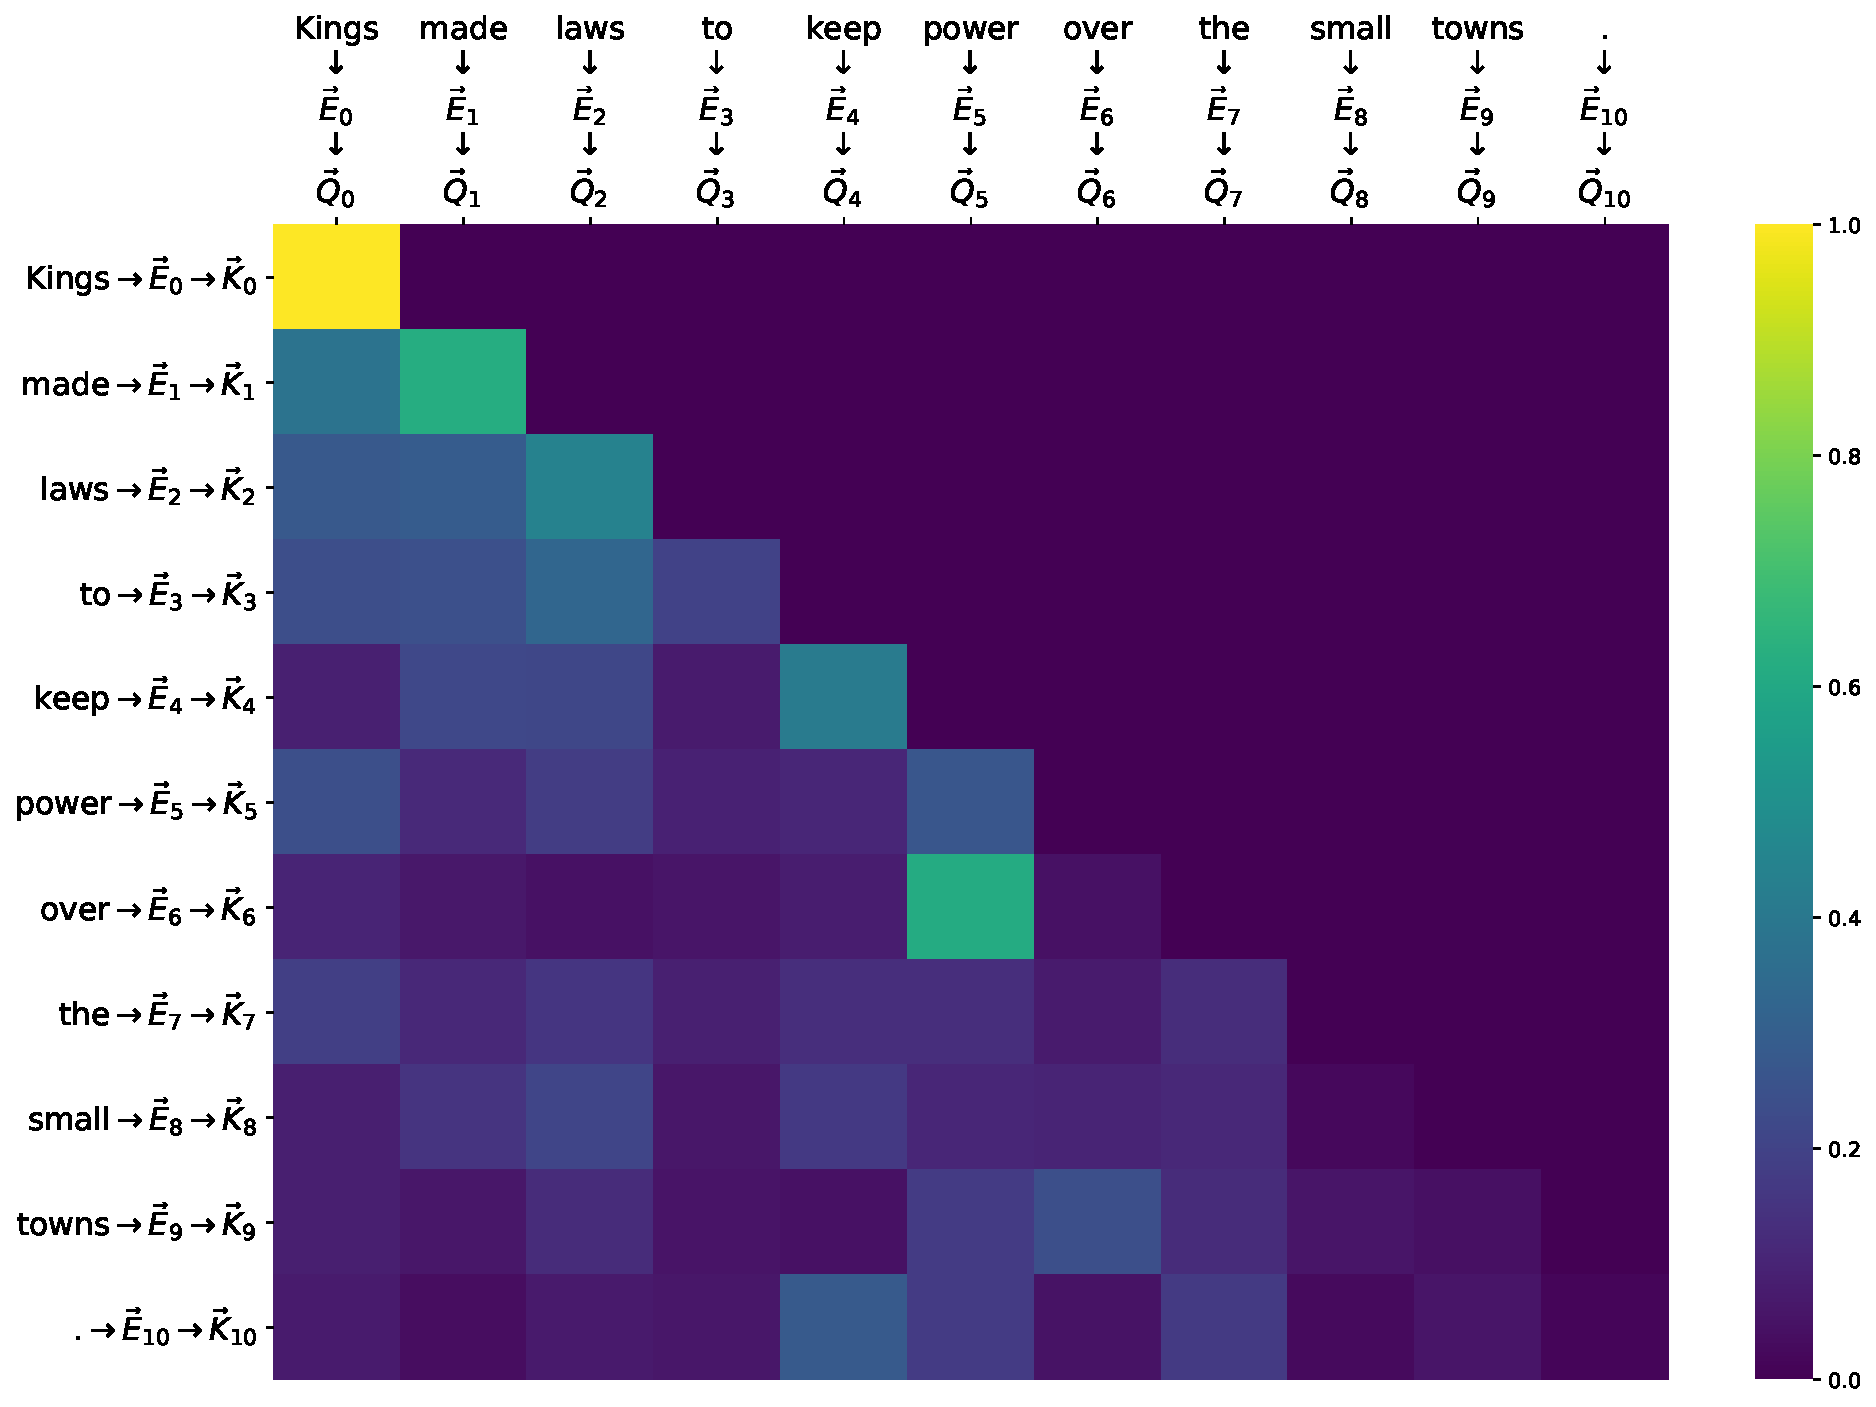
\includegraphics[width=\linewidth]{images/mod_attn.pdf}
  \end{minipage}
\caption{Illustration of the attention patterns from the first attention head in the first layer of GPT-2, for the input text: 
\textit{''Kings made laws to keep power over the small towns.``} The left plot shows the raw attention scores ($QK^T$), while 
the right plot displays the masked and scaled attention weights after applying the softmax function, i.e., 
$\text{softmax}\left(\frac{QK^T}{\sqrt{d_k}}\right)$.}
\end{figure}

\subsubsection{Multi-Head Attention}
The process described above outlines a single ''head`` of attention, where each word attends to other words 
based on their relevance. However, in practice, we use multi-head attention, which runs multiple attention 
mechanisms in parallel, each with its own learned query, key, and value matrices.\newline
The benefit of multi-head attention is that it allows the model to focus on different aspects of the input 
simultaneously. For instance, one head might focus on syntactic relationships, while another might focus on 
semantic meanings, and yet another could capture long-range dependencies. This parallel processing allows 
the transformer to learn richer, more nuanced representations.\newline
To make this process more efficient, each attention head typically uses smaller key, value, and query 
matrices. After the attention 
outputs are computed using these smaller matrices, the results from all heads are concatenated and passed 
through a linear layer to combine them. The formula for a Multi-Head attention block with $k$ heads is given by 
$$\text{MultiHead}(Q,K,V)=\text{Concat}[\text{head}_1,\dots,\text{head}_k]W_O$$
where $W_O$ is the learnable output projection matrix of dimension $(k\cdot d_h) \times d_\text{model}$
with $d_h$ being the dimensionality of the value vectors (the same as the dimensionality of each head's output) and
$d_\text{model}$  the final desired output dimensionality of the multi-head attention (usually equal to the 
model's embedding size).
\begin{figure}[H]
    \centering
    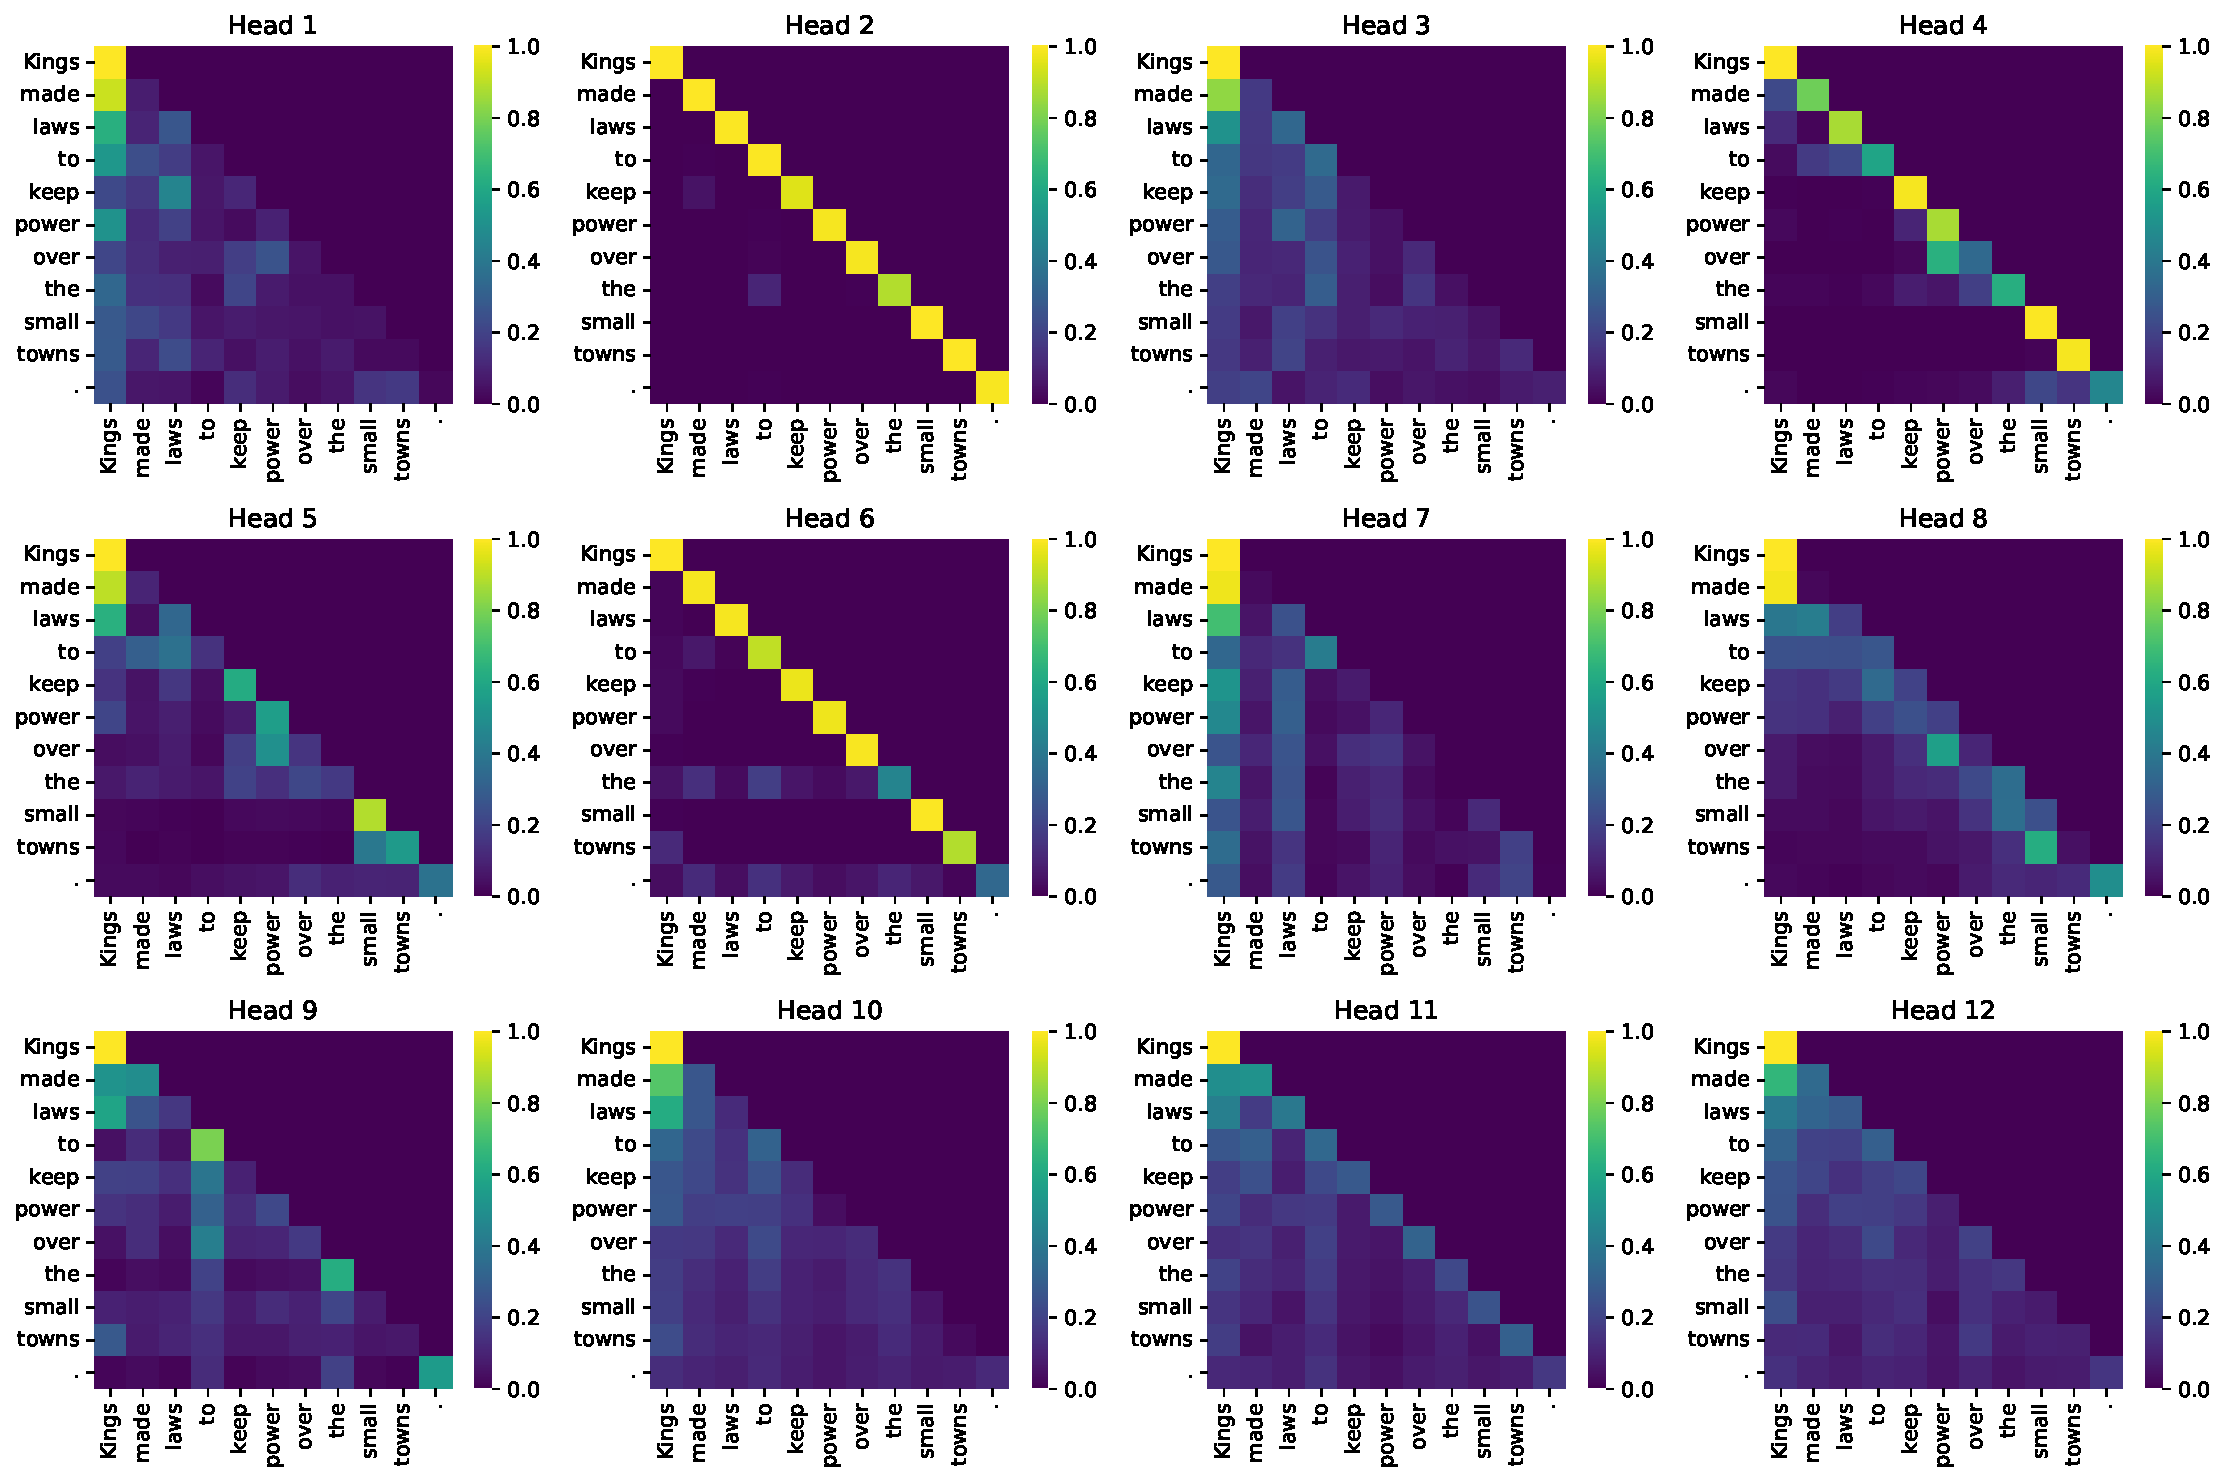
\includegraphics[width=0.8\linewidth]{images/multi_head_attn.pdf}
  \caption{Illustration of the attention patterns from all heads in the first layer of GPT-2 for the sentence: \textit{"Kings 
  made laws to keep power over the small towns."}}
\end{figure}

\subsection{Feedforward Neural Network and Add \& Norm}
The Feedforward Neural Network (FNN) in Transformers is a simple multi-layer perceptron (MLP) composed of fully connected 
layers with ReLU activations.\newline
The "Add" operation refers to residual (skip) connections, which are critical for stabilizing deep networks. Without them, 
models can suffer from vanishing or exploding gradients, making training inefficient or unstable. Residual connections allow 
gradients to flow more directly through the network and help mitigate the degradation problem, where adding more layers leads 
to worse performance. \newline 
Normalization further stabilizes training by ensuring that inputs to each layer are centered and appropriately scaled. While 
Batch Normalization (BN) normalizes across the batch dimension, it is less suitable for Transformer architectures, which often 
work with variable-length sequences and small batch sizes. Instead, Transformers use Layer Normalization (LN), which 
normalizes across feature dimensions for each individual sequence. This approach is more robust in the context of sequence modeling.

\subsection{Modifications to the Vanilla Transformer}
While the original transformer architecture has demonstrated strong performance across a range of tasks, it also faces certain 
limitations particularly when modeling long sequences. In this section, we examine follow-up work that addresses these issues.


\subsubsection{Transformer-XL}
Transformers are capable of learning long-term dependencies, but they are limited by a 
fixed-length context when applied to language modelling tasks. Transformer-XL 
\cite{dai2019transformerxlattentivelanguagemodels} proposes an 
architecture that extends this capability by enabling the learning of dependencies beyond 
a fixed length, without disrupting temporal coherence. This is achieved by incorporating a 
memory mechanism into the transformer model.\newline
The approach begins by splitting the input into segments, denoted as $X_i$. If we were to 
process these segments using a standard transformer model, there would be no attention 
between them, as illustrated in Figure \ref{fig:vanilla}.\newline 
To overcome this, Transformer-XL concatenates the hidden states from the previous segment with the current input at every 
transformer layer. These past states are treated as fixed memory i.e. gradients are not propagated through 
them allowing efficient reuse without increasing memory cost during backpropagation. This approach is illustrated in 
Figure \ref{fig:xl}.
\begin{figure*}[!h]
	\begin{subfigure}[b]{0.292\linewidth}
		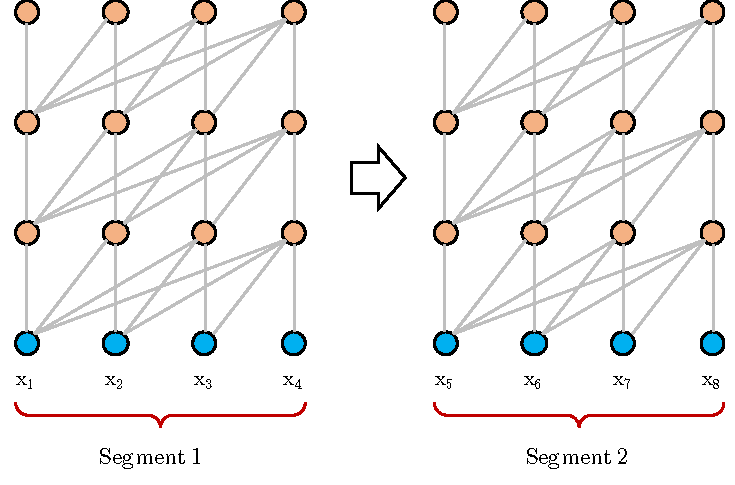
\includegraphics[width=\textwidth]{images/vanilla-train.pdf}
		\caption{\small Train phase.}
		\label{fig:vanilla-train}
	\end{subfigure}
	\rulesep
	\begin{subfigure}[b]{0.69\linewidth}
		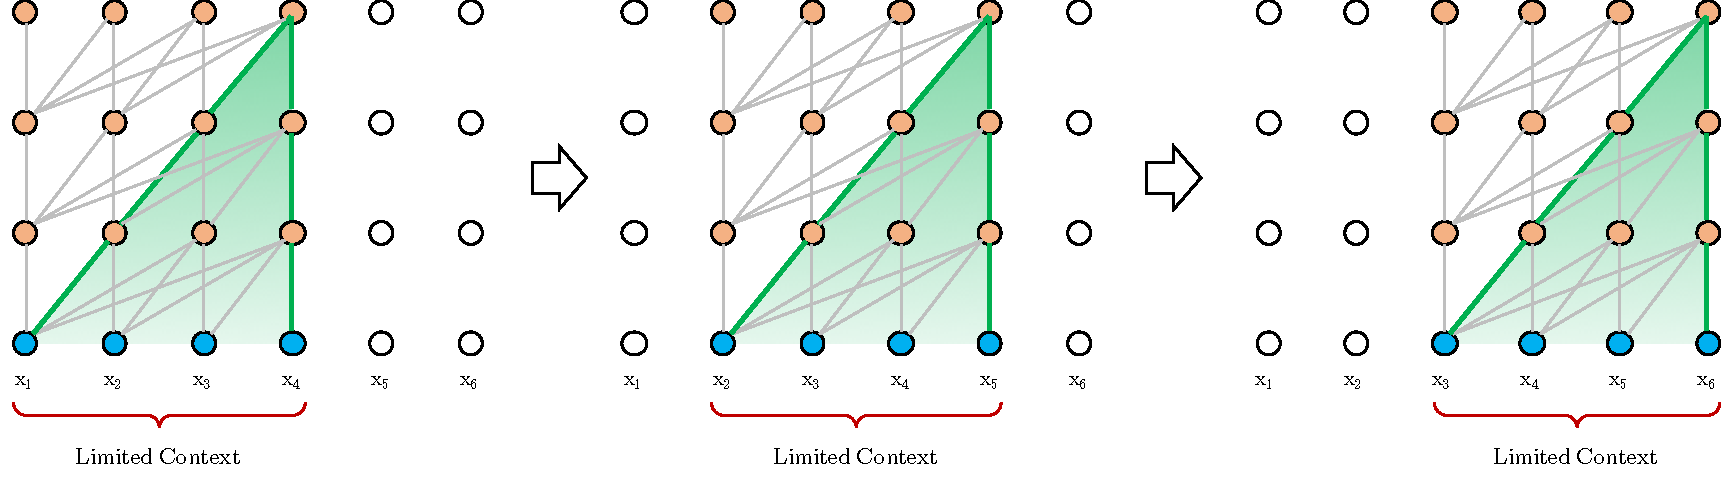
\includegraphics[width=\textwidth]{images/vanilla-eval.pdf}
		\caption{\small Evaluation phase.}
		\label{fig:vanilla-eval}
	\end{subfigure}
	\caption{\small Illustration of the vanilla transformer model with a segment length 4. \cite{dai2019transformerxlattentivelanguagemodels}}
	\label{fig:vanilla}
\end{figure*}

\begin{figure*}[!h]
	\begin{subfigure}[b]{0.62\linewidth}
		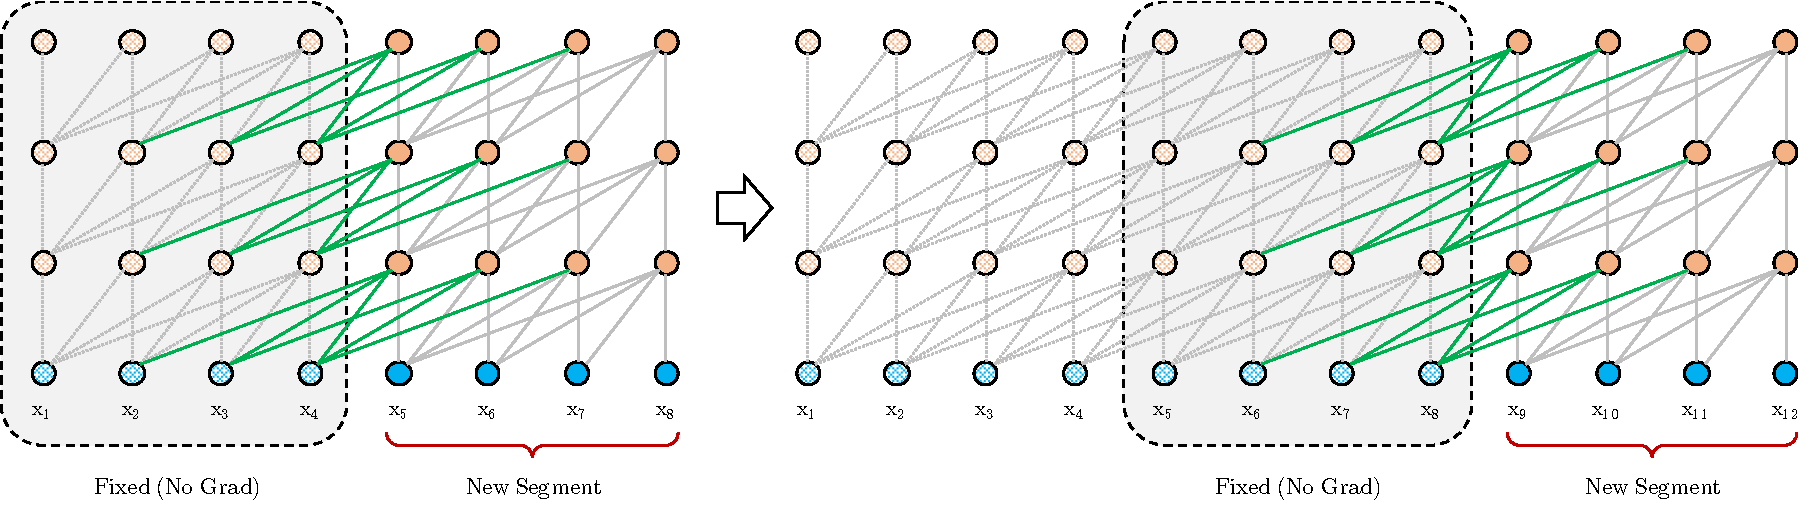
\includegraphics[width=\textwidth]{images/xl-train.pdf}
		\caption{\small Training phase.}
		\label{fig:xl-train}
	\end{subfigure}
	\rulesep
	\begin{subfigure}[b]{0.35\linewidth}
		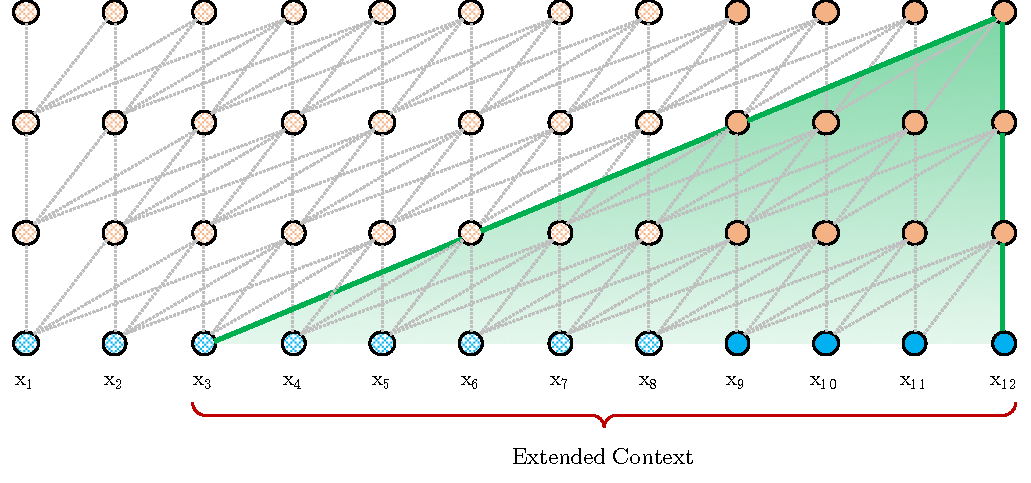
\includegraphics[width=\textwidth]{images/xl-eval.pdf}
		\caption{\small Evaluation phase.}
		\label{fig:xl-eval}
	\end{subfigure}
	\caption{\small Illustration of the Transformer-XL model with a segment length 4. \cite{dai2019transformerxlattentivelanguagemodels}}
	\label{fig:xl}
\end{figure*}
However, this modification introduces a new challenge: absolute positional encodings used in vanilla transformers cannot 
correctly handle segment-level continuity. For example, tokens $X_1^1$ (from one segment) and $X_1^2$ (from the next) would 
receive identical positional encodings, despite being temporally distinct. This breaks the sequence order and confuses the 
model.\newline
To solve this, Transformer-XL replaces absolute positional encodings with relative positional encodings. This allows the model 
to compute attention based on the relative distance between tokens, preserving the temporal relationships across segments. For
implementation details, refer to Section 3.3 in the original paper \cite{dai2019transformerxlattentivelanguagemodels}.

\subsubsection{Stabilizing Transformers for Reinforcement Learning}
Despite their success in NLP and vision, vanilla transformers and their memory-augmented variants 
like Transformer-XL initially performed poorly in reinforcement learning (RL) settings. For instance, 
\cite{mishra2018simpleneuralattentivemetalearner} found that standard transformers failed on even basic 
bandit problems and tabular Markov Decision Processes (MDPs), suggesting that transformers may not be 
well-suited for RL without further adaptation.\newline 
To address this, \cite{parisotto2019stabilizingtransformersreinforcementlearning} proposed modifications that significantly 
improve transformer stability and performance in RL. Their work builds on Transformer-XL and introduces two key changes.

\paragraph{1. TrXL-I: Input-Normalized Transformer-XL} The first modification is reordering the application of layer 
normalization. Instead of applying it before and after each submodule (as in the original transformer), it is applied only to 
the inputs. This reordering creates an identity map from the input of the transformer at the first layer to the output at the 
last layer, unlike the canonical transformer, which applies multiple layer normalization operations that non-linearly 
transform the state encoding.\newline
TrXL-I shows a significant improvement in stability and performance over TrXL. One 
hypothesis for this improvement is that, with the initialization of submodules producing 
values near zero, the state encoding is passed untransformed to the policy and value 
heads. This allows the agent to learn a Markovian policies first e.g. 
$\pi(a | s_1, ..., s_n) \approx \pi(a | s_n)$ before gradually incorporating longer-term memory, 
which aligns with how agents typically learn: basic behaviors precede memory-dependent 
strategies.\cite{parisotto2019stabilizingtransformersreinforcementlearning}

\paragraph{2. GTrXL: Gated Transformer-XL} To further stabilize learning, the authors replace standard residual connections 
with gated residual layers, inspired by gating mechanisms in LSTMs. This results in the Gated Transformer-XL (GTrXL) 
architecture. Gating enables dynamic control over how much information is retained or suppressed at each layer, improving both 
optimization and generalization.\newline 
For a detailed explanation of how the gating block is defined, refer to the original paper 
\cite{parisotto2019stabilizingtransformersreinforcementlearning}. The authors explore various gating functions—similar to 
A helpful supplementary resource on gating mechanisms in neural networks can be found 
\href{https://medium.com/autonomous-agents/a-math-deep-dive-on-gating-in-neural-architectures-b49775810dde}{see})

\begin{figure}[H]
    \centering
    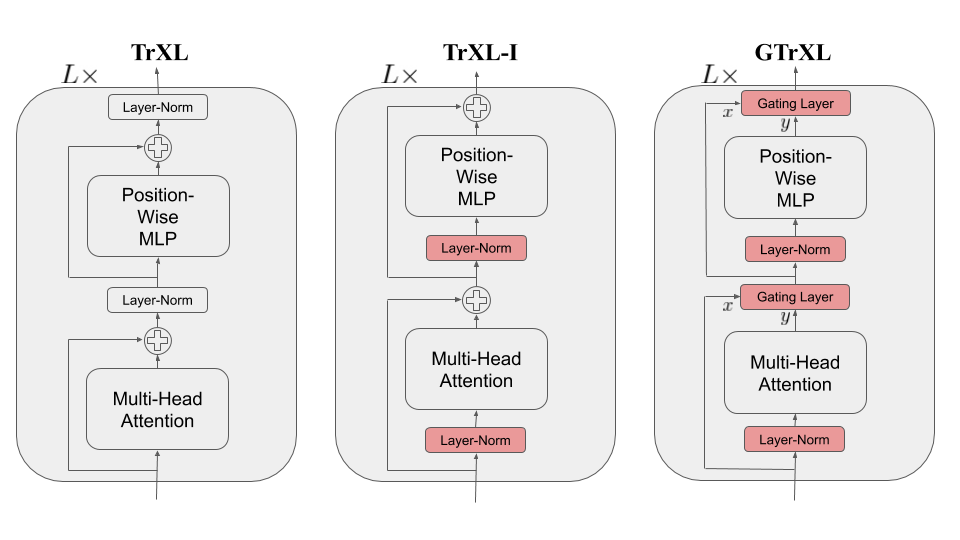
\includegraphics[width=0.7\linewidth]{images/gtrxl.png}
    \caption{Visualisation of the modified Transformer-XL block from \cite{parisotto2019stabilizingtransformersreinforcementlearning}}
    \label{fig:gtrxl}
\end{figure}

\subsection{Transformers in RL}
While this section does not cover all transformer-based approaches in reinforcement learning, several notable works are worth 
highlighting for further reading. Decision Transformer \cite{chen2021decisiontransformerreinforcementlearning} introduced a novel 
framing of reinforcement learning as a sequence modeling problem, treating trajectories as input-output sequences. More recently, 
PoliFormer \cite{poliformer2024} demonstrated that scaling on-policy RL with transformer architectures can produce highly capable 
agents, particularly in navigation tasks.

\subsection{Pros and Cons of Transformers in RL}
Transformer-based models in RL offer several advantages. They are well-suited for evaluating memory and credit assignment 
capabilities, and they tend to perform strongly on tasks that require long-term memory. However, they do not inherently improve 
long-term credit assignment and often suffer from poor sample efficiency. Additionally, many existing RL benchmarks that aim to 
test memory or credit assignment often conflate the two or rely on tasks with predominantly short-term dependencies, limiting the 
insights that can be drawn about transformers' strengths in truly long-horizon settings.

\subsection{Resources}
There are several excellent resources for learning about transformers. A particularly insightful video series is the Neural 
Networks series by 3Blue1Brown, which includes a well-explained introduction to transformers \cite{3ble1brownNN}. Another highly 
recommended resource is Lilian Weng’s blog post, Attention? Attention! \cite{weng2018attention}, which provides a clear and 
intuitive breakdown of the underlying mechanisms.


%\begin{table}[H]
%\begin{tabularx}{\linewidth}{>{\parskip1ex}X@{\kern4\tabcolsep}>{\parskip1ex}X}
%\toprule
%\hfil\bfseries Transformer
%&
%\hfil\bfseries RNN
%\\\cmidrule(r{3\tabcolsep}){1-1}\cmidrule(l{-\tabcolsep}){2-2}

%% PROS, separated by empty line or \par
%Transformers, using self-attention, process all tokens simultaneously, speeding up training and inference. \par
%Transformers' self-attention allows tokens to attend to each other directly, efficiently capturing long-range dependencies. %\par

%&
%
%% CONS, separated by empty line or \par
%RNNs process data sequentially, limiting parallelization and slowing training. \par
%RNNs struggle with long sequences due to vanishing gradients. \par

%\\\bottomrule
%\end{tabularx}
%\end{table}

